% !TeX root = ../navier-stokes-manuscript.tex
% ============================================================
% 1.6 A Comparison with Euler
% ============================================================
\subsection{A Comparison with Euler}\label{sub:AComparisonWithEuler}

Couette flow gives the continuous participation picture in its simplest physical form.
Place fluid between two parallel plates a distance \(h\) apart, move the upper plate tangentially with velocity \(U_+e_1\), and move the lower plate with velocity \(U_-e_1\), where \(U_-\neq U_+\).
The steady velocity between them is
\[
  u_C(x)
  =
  \left(
    U_-+\frac{U_+-U_-}{h}x_3
  \right)e_1,
  \qquad
  0<x_3<h,
  \qquad
  p=p_0.
\]
Every layer takes an intermediate tangential speed, and neighbouring layers differ by the finite shear
\[
  \partial_3(u_C)_1
  =
  \frac{U_+-U_-}{h}.
\]
The plates maintain the physical laboratory flow, while the profile lets us see the continuous velocity relation carried through the fluid between them.
\Cref{fig:CouetteFlow} draws that relation.

% !TeX root = ../../navier-stokes-manuscript.tex
\begin{figure}[!htbp]
  \centering
  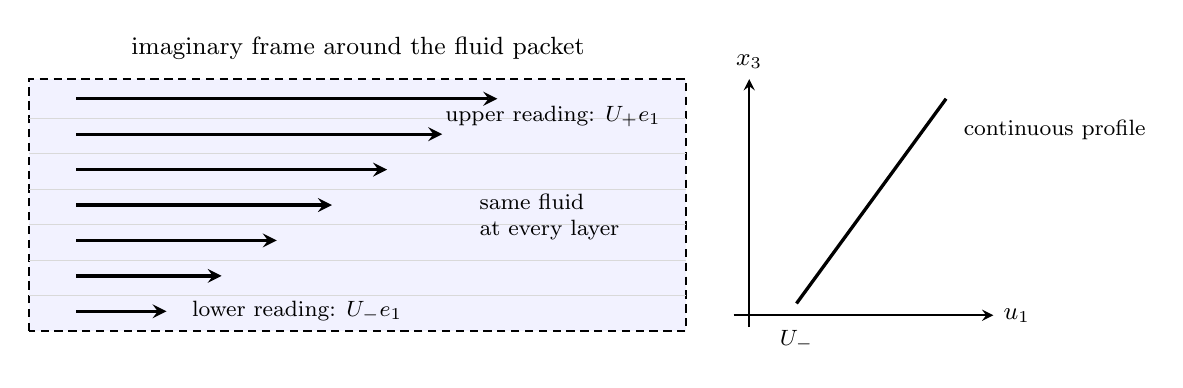
\begin{tikzpicture}[
    x=1cm,
    y=1cm,
    >=stealth,
    velocity/.style={->,very thick},
    smalllabel/.style={font=\small},
    tinylabel/.style={font=\footnotesize}
  ]
    \fill[blue!5]
      (0.50,0.65) rectangle (8.85,3.85);
    \draw[densely dashed,thick]
      (0.50,0.65) rectangle (8.85,3.85);

    \foreach \y in {1.10,1.55,2.00,2.45,2.90,3.35}
      \draw[black!15] (0.50,\y) -- (8.85,\y);

    \draw[velocity] (1.10,0.90) -- (2.25,0.90);
    \draw[velocity] (1.10,1.35) -- (2.95,1.35);
    \draw[velocity] (1.10,1.80) -- (3.65,1.80);
    \draw[velocity] (1.10,2.25) -- (4.35,2.25);
    \draw[velocity] (1.10,2.70) -- (5.05,2.70);
    \draw[velocity] (1.10,3.15) -- (5.75,3.15);
    \draw[velocity] (1.10,3.60) -- (6.45,3.60);

    \node[tinylabel,anchor=east] at (8.65,3.38)
      {upper reading: \(U_+e_1\)};
    \node[tinylabel,anchor=west] at (2.45,0.90)
      {lower reading: \(U_-e_1\)};
    \node[smalllabel,anchor=south] at (4.68,3.98)
      {imaginary frame around the fluid packet};
    \node[tinylabel,align=left,anchor=west] at (6.10,2.10)
      {same fluid\\at every layer};

    \draw[->,thick] (9.65,0.70) -- (9.65,3.85)
      node[above,smalllabel] {\(x_3\)};
    \draw[->,thick] (9.45,0.85) -- (12.75,0.85)
      node[right,smalllabel] {\(u_1\)};
    \draw[very thick] (10.25,1.00) -- (12.15,3.60);
    \node[tinylabel,anchor=north] at (10.25,0.78) {\(U_-\)};
    \node[tinylabel,anchor=west] at (12.25,3.20)
      {continuous profile};
  \end{tikzpicture}
  \caption{Continuous shear imagined inside one fluid packet.
  The dashed outline is only an observation frame.
  Every layer takes an intermediate velocity, so the one velocity field remains smooth across the packet.}
  \label{fig:CouetteFlow}
\end{figure}


Now take one packet of the unforced fluid and draw two imaginary horizontal lines through it at the same separation.
The lines mark two locations inside the packet and supply no walls, plates, or external forcing.
Assign \(U_-e_1\) near the lower line and \(U_+e_1\) near the upper line, and imagine the fluid took on these properties of the Couette profile between them.
The same continuous formula then describes the packet locally.

The equation class of this imagined packet follows from its geometry.
Because the velocity points in the \(e_1\)-direction and varies linearly in the \(x_3\)-direction,
\[
  \nabla\cdot u_C=0,
  \qquad
  (u_C\cdot\nabla)u_C=0,
  \qquad
  \Delta u_C=0,
  \qquad
  \nabla p=0.
\]
It satisfies the local Euler momentum law and the local fixed-viscosity \NavierStokes{} momentum law at the same time.
Positive viscosity is present.
This linear profile has no spatial curvature for the Laplacian to act on.
The nonzero shear by itself does not become a nonzero bulk viscous force.

Keep the same packet, the same two imaginary lines, and the same assigned velocities.
Change how the one fluid joins them.
Let all fluid below a middle plane move with \(U_-e_1\) and all fluid above it move with \(U_+e_1\), leaving no intermediate velocities across that internal surface.
The motion now has the rigid slip pattern of two boards passing one another.
The boards describe the behaviour being imagined; the physical object remains one fluid packet.
\Cref{fig:BoardLikeSlip} draws this second velocity relation.

% !TeX root = ../../navier-stokes-manuscript.tex
\begin{figure}[!htbp]
  \centering
  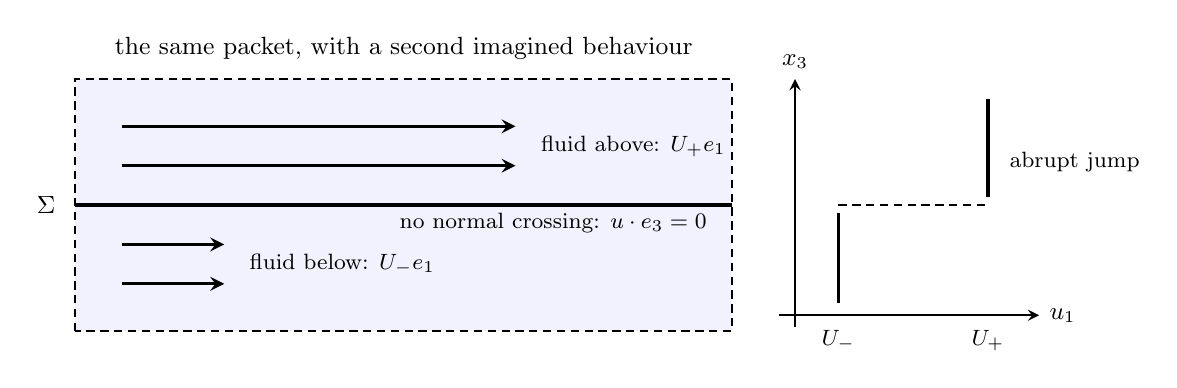
\begin{tikzpicture}[
    x=1cm,
    y=1cm,
    >=stealth,
    velocity/.style={->,very thick},
    smalllabel/.style={font=\small},
    tinylabel/.style={font=\footnotesize}
  ]
    \fill[blue!5]
      (0.50,0.65) rectangle (8.85,3.85);
    \draw[densely dashed,thick]
      (0.50,0.65) rectangle (8.85,3.85);
    \draw[very thick] (0.50,2.25) -- (8.85,2.25);
    \node[smalllabel,anchor=east] at (0.38,2.25) {\(\Sigma\)};

    \draw[velocity] (1.10,1.25) -- (2.40,1.25);
    \draw[velocity] (1.10,1.75) -- (2.40,1.75);
    \draw[velocity] (1.10,2.75) -- (6.10,2.75);
    \draw[velocity] (1.10,3.25) -- (6.10,3.25);

    \node[tinylabel,anchor=west] at (6.30,3.00)
      {fluid above: \(U_+e_1\)};
    \node[tinylabel,anchor=west] at (2.60,1.50)
      {fluid below: \(U_-e_1\)};
    \node[smalllabel,anchor=south] at (4.68,3.98)
      {the same packet, with a second imagined behaviour};
    \node[tinylabel,anchor=east] at (8.65,2.02)
      {no normal crossing: \(u\cdot e_3=0\)};

    \draw[->,thick] (9.65,0.70) -- (9.65,3.85)
      node[above,smalllabel] {\(x_3\)};
    \draw[->,thick] (9.45,0.85) -- (12.75,0.85)
      node[right,smalllabel] {\(u_1\)};
    \draw[very thick] (10.20,1.00) -- (10.20,2.15);
    \draw[very thick] (12.10,2.35) -- (12.10,3.60);
    \draw[densely dashed] (10.20,2.25) -- (12.10,2.25);
    \node[tinylabel,anchor=north] at (10.20,0.78) {\(U_-\)};
    \node[tinylabel,anchor=north] at (12.10,0.78) {\(U_+\)};
    \node[tinylabel,anchor=west] at (12.25,2.80)
      {abrupt jump};
  \end{tikzpicture}
  \caption{Board-like motion imagined inside the same fluid packet.
  The dashed outline is not a wall, and the two regions are not separate bodies.
  The one velocity field jumps tangentially across \(\Sigma\), so this profile is nonsmooth even though its normal flow remains zero.}
  \label{fig:BoardLikeSlip}
\end{figure}


The velocity jump makes smoothness fail visibly.
Class membership still has to be decided by the equations.
Euler and \NavierStokes{} must test the same proposed velocity, pressure, incompressibility, and nonlinear momentum transport.
Across a jump, the common laws are read in divergence form:
\[
  \begin{aligned}
  \text{Euler:}\qquad
  &\partial_tu+\nabla\cdot(u\otimes u)+\nabla p=0,\\
  \text{\NavierStokes:}\qquad
  &\partial_tu+\nabla\cdot(u\otimes u)+\nabla p=\nu\Delta u,
  \qquad \nu>0,
  \end{aligned}
\]
with \(\nabla\cdot u=0\) in both cases.
The shared requirements come first, because viscosity can separate the two classes only after the rest of the proposed field has been held fixed.

Let the internal surface be \(\Sigma=\{x_3=0\}\), with normal \(e_3\), and set
\[
  u(x)
  =
  \begin{cases}
    U_-e_1, & x_3<0,\\
    U_+e_1, & x_3>0,
  \end{cases}
  \qquad
  p(x)=p_0.
\]
Its jump
\[
  [u]=(U_+-U_-)e_1
\]
lies completely along the interface.
Writing \(\delta_\Sigma\) for unit surface mass on \(\Sigma\), the divergence defect is
\[
  \nabla\cdot u
  =
  [u]\cdot e_3\,\delta_\Sigma
  =0.
\]
There is no source, sink, or mass flux through the plane.

The same tangential geometry removes the nonlinear momentum flux across the interface.
On either side,
\[
  (u\otimes u)e_3
  =
  u(u\cdot e_3)
  =0,
\]
so \(\nabla\cdot(u\otimes u)=0\) as a distribution.
The field is stationary and the pressure is constant, which also gives \(\partial_tu=0\) and \(\nabla p=0\).
Every term shared by Euler and \NavierStokes{} vanishes for this proposed motion.

This stationary tangential discontinuity is a planar vortex sheet.
It is a local distributional weak solution of the incompressible Euler equations.
The velocities stay finite on the two sides, while the missing intermediate shear is concentrated on the interface:
\[
  \nabla\times u
  =
  (U_+-U_-)e_2\,\delta_\Sigma.
\]
Euler admits the board-like behaviour locally because its law has no term that compares the two tangential velocities through spatial curvature.

Fixed positive viscosity makes that comparison unavoidable.
For the unchanged stationary field,
\[
  \Delta u
  =
  (U_+-U_-)e_1\,\partial_3\delta_\Sigma.
\]
The left side of the momentum equation is still zero while \(\nu\Delta u\) is not.
Pressure cannot absorb the unmatched viscous distribution because
\[
  \nabla\times(\nu\Delta u)
  =
  \nu(U_+-U_-)e_2\,\partial_3^2\delta_\Sigma
  \neq0,
  \qquad
  \nabla\times\nabla p=0
\]
for every scalar pressure distribution \(p\).
The fixed velocity--pressure candidate belongs locally to the Euler class and fails the fixed-positive-viscosity \NavierStokes{} equation.
Viscosity has distinguished the two laws without changing the fluid pattern offered to them.

Allowing the jump to evolve shows what the viscous fluid does instead.
Keep the planar form
\[
  u(x,t)=(U(x_3,t),0,0),
  \qquad
  p=p_0.
\]
Incompressibility remains automatic and nonlinear transport remains zero, so the two equations reduce to
\[
  \text{Euler:}\quad \partial_tU=0,
  \qquad
  \text{\NavierStokes:}\quad \partial_tU=\nu\partial_3^2U.
\]
Euler leaves the tangential profile fixed in this ansatz.
\NavierStokes{} turns the same initial profile into one-dimensional heat flow.
Starting from
\[
  U(x_3,0)
  =
  \begin{cases}
    U_-, & x_3<0,\\
    U_+, & x_3>0,
  \end{cases}
\]
the solution at every \(t>0\) is
\[
  U(x_3,t)
  =
  \frac{U_-+U_+}{2}
  +
  \frac{U_+-U_-}{2}
  \operatorname{erf}\!\left(\frac{x_3}{2\sqrt{\nu t}}\right).
\]
The sharp interface immediately becomes a continuous layer with thickness comparable to \(\sqrt{\nu t}\).
Positive viscosity communicates tangential momentum across the internal surface and fills in the velocities that the stationary board-like picture omitted.

This returns us to the Couette profile with the physical distinction intact.
The linear Couette-like packet has nonzero shear and zero Laplacian in its interior, so it creates no bulk viscous residual there.
The step has a distributional second derivative, so fixed positive viscosity cannot leave it stationary.
Actual Couette plates continually maintain the laboratory shear, while the imaginary lines in the packet provide no such external action.

The calculation is local, and class membership still carries the whole-space requirements.
The infinite planar sheet does not decay, has infinite kinetic energy on \(\mathbb R^3\), lies outside \(H^1\), and is not the continuation generated by the fixed datum in \cref{sub:ClassMembershipAndParticipation}.
It is an exact local comparison between the Euler and fixed-viscosity laws.
Its infinite-energy whole-space geometry prevents it from being a Millennium counterexample.
Even with those global defects set aside, the nonzero viscous residual already gives
\[
  \neg\operatorname{Member}(Q)
\]
for the stationary sheet offered as a \NavierStokes{} continuation.

In this example the visible nonsmoothness is the tangential slip.
The slip omits the response that fixed positive viscosity demands across the internal surface.
That loss of viscous participation leaves the proposed field Euler-only in the local comparison and forces \NavierStokes{} class exit.
Here the first disagreement occurs in velocity itself, where the two sides of the packet carry incompatible values.
A more subtle loss can keep velocity finite and continuous while acceleration, jerk, a spatial gradient, or some higher mixed derivative ceases to take part in one smooth response.
Following that possibility requires opening the response of the same fluid beyond its lowest velocity reading.
